\begin{figure*}[!ht]
    \centering
    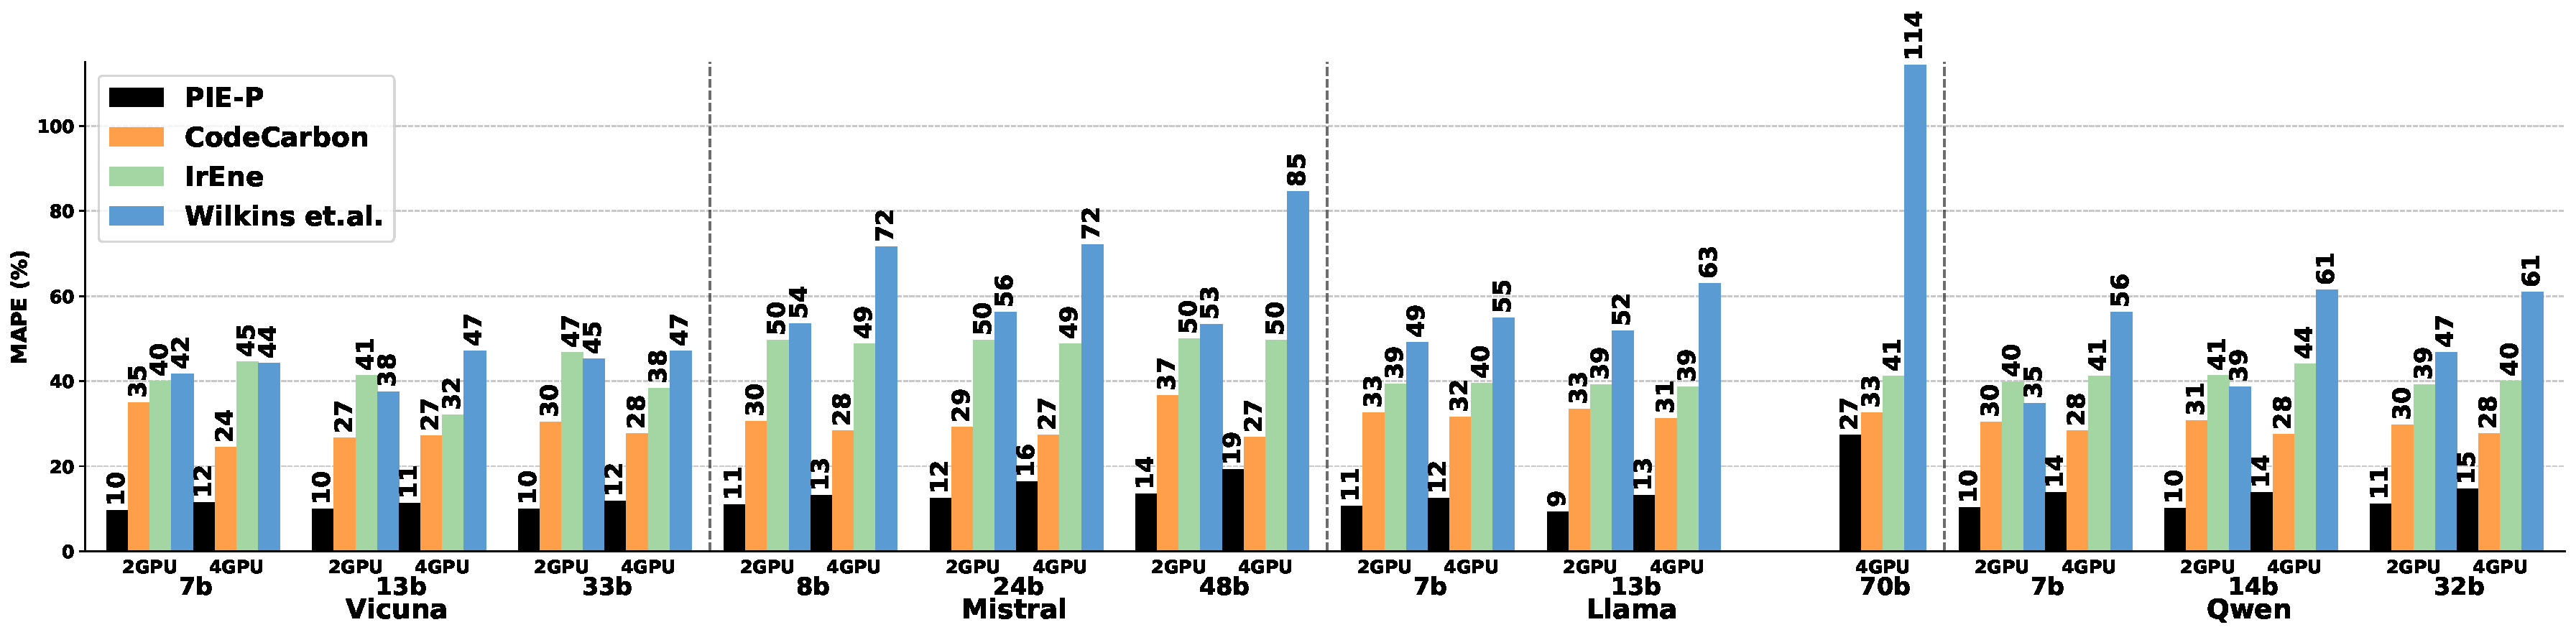
\includegraphics[width=\textwidth]{figures/mape_all_model_families.pdf}
    \vspace{-24pt}
    \caption{MAPE results across model families for \sys{} and the baselines under tensor parallelism on A6000.}
    \label{fig:mape_comparison}
    \vspace{-9pt}
\end{figure*}

\begin{figure*}[!t]
\centering
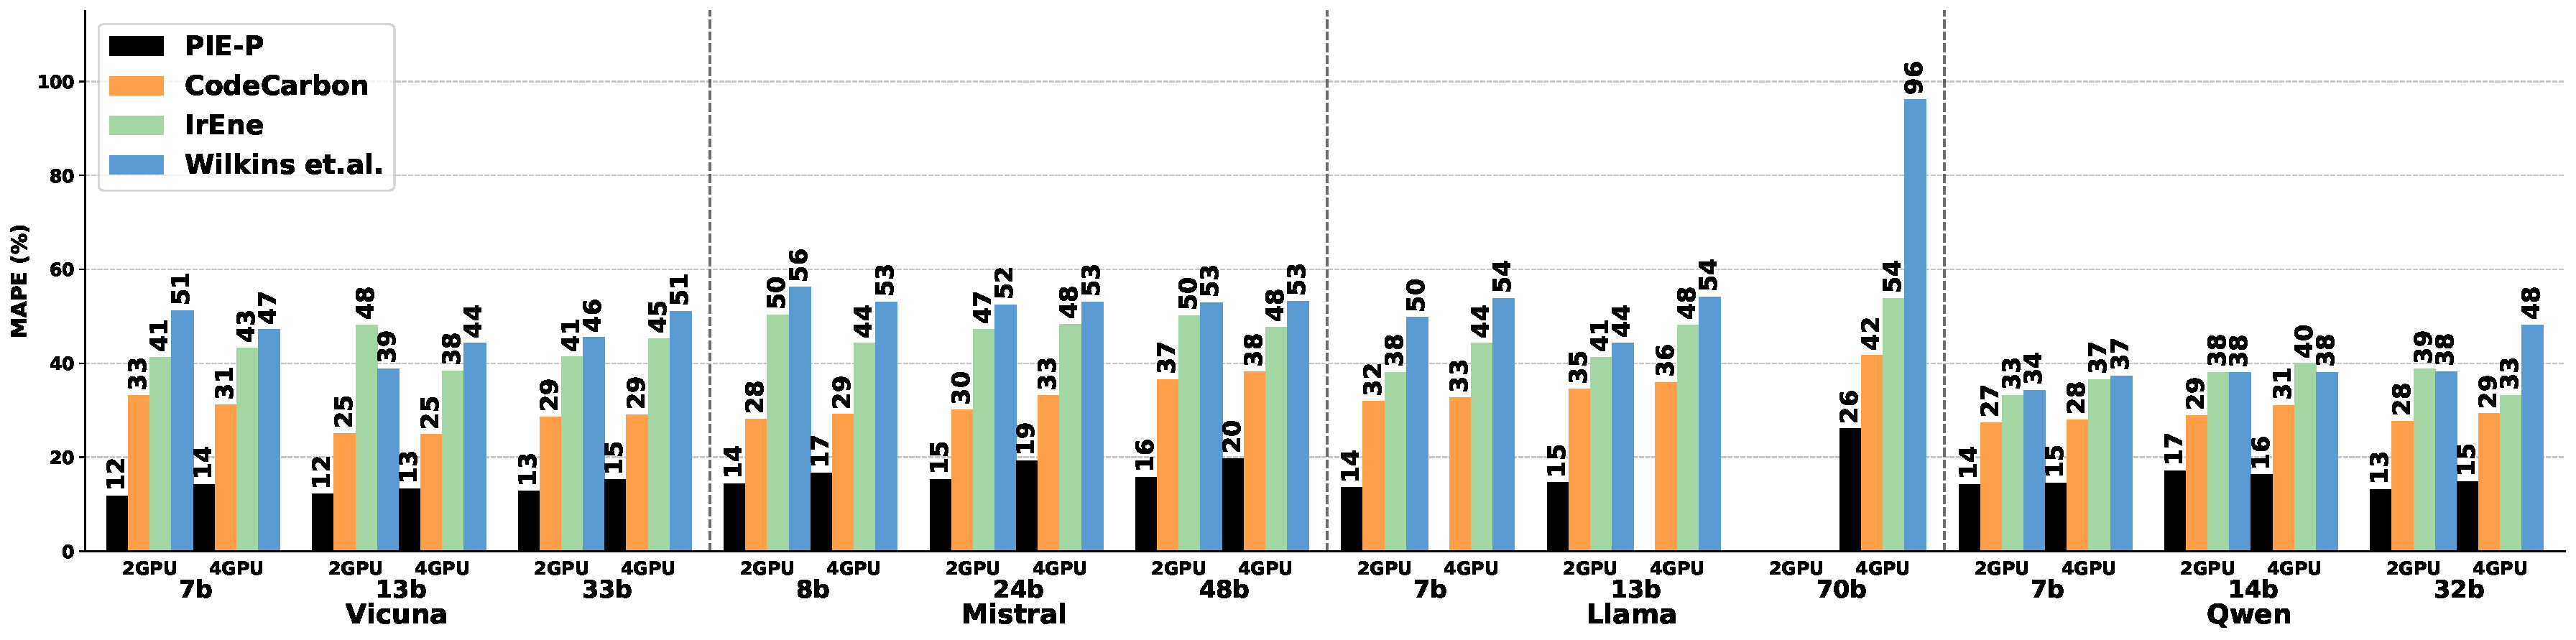
\includegraphics[width=\textwidth]{figures/b40_mape_tensor_parallelism_with_codecarbon.pdf}
\vspace{-24pt}
\caption{MAPE results across model families for \sys{} and the baselines under tensor parallelism on B40.}
\label{fig:b40_mape_tensor_parallelism}
\vspace{-18pt}
\end{figure*}

Our evaluation demonstrates \sys{}'s effectiveness across four LLM model families across varying sizes (7B--70B): Vicuna, Mistral, Llama, and Qwen~\cite{vicuna, jiang2023mistral7b, touvron2023llama, qwen}.
We experiment on three different hardware platforms that use different communication modes (NVLink and PCIe) across the three widely employed parallelization strategies (tensor, pipeline, and data). We evaluate all three forms of parallelism, while using tensor parallelism for the most extensive analysis because individual model operators are partitioned across GPUs and collective communication is repeatedly interleaved with computation inside Transformer blocks. This makes its communication and synchronization behavior substantially more involved than the stage-boundary transfers in pipeline parallelism and the less frequent communication in our data-parallel inference setup.

\subsection{Evaluation Methodology}
\label{ss:esetup}
We conducted experiments on three hardware platforms:
(1) NVIDIA RTX A6000;
(2) NVIDIA B40; and
(3) NVIDIA H200.
Platform (1) uses an AMD EPYC Milan 7543P 32-core CPU with four A6000 GPUs over PCIe 4.0. Platforms (2) and (3) use an Intel Xeon 6 6530P 32-core CPU with PCIe 4.0 for B40 and NVLink-connected GPUs for H200.
Ground-truth system power/energy is measured using an external Watts Up Pro monitor (platform~1) and IPMI/BMC power readings (platforms 2,3).

\anurag{Appendix - E Methodology: Training}
\review{\smallskip\noindent\textbf{Training methodology.} We train \sys{} hierarchically: module-level predictors are learned first and their predictions are then composed into model-level energy. We use 3-fold cross-validation at the module level with a 70\%/30\% train/test split. Each module type (e.g., Self-Attention, MLP, and AllReduce) is sampled $10{,}000$ times to build a robust dataset. A sample is an aggregate measurement formed by running the module $100{,}000$ times under a fixed model and GPU configuration. For every sample, runtime features across the participating GPUs are reduced to their mean, standard deviation, minimum, and maximum values to capture both the overall activity level and cross-GPU imbalance, and these statistics are combined with the structural features in Table~\ref{tab:features}.}

\review{To expose the predictors to different operating regimes, we profile batch sizes 8, 16, 32, and 64 and output sequence lengths 512 and 1024. We use DeepSpeed~\cite{deepspeed} for tensor-, pipeline-, and data-parallel inference. We evaluate generalization using leave-one-out experiments because a useful predictor should transfer to models that were not present in its training measurements. In leave-one-variant-out evaluation, an entire model variant is excluded and predicted using module-level predictors learned from the remaining variants in the same family. In leave-one-family-out evaluation, all variants of one family are excluded from training, providing a stricter test of transfer across model architectures.}

\review{Our primary tensor-parallel evaluation covers the complete model suite on the A6000 and B40 platforms. We then use representative experiments on the H200 and in the additional generalization analyses to test whether the same decomposition and feature design continue to work across different hardware and model settings. We do not repeat every experiment on every model--hardware combination; instead, the full suite establishes the main result and the representative experiments test the relevant generalization dimensions.}

\smallskip\noindent\textbf{Baselines and comparison variants.} We compare \sys{} against the following prediction and measurement baselines, together with controlled variants that isolate the contribution of its design choices. \\
\noindent\textbf{\be{IrEne}~\cite{irene}:} A hierarchical energy prediction framework for single-GPU execution and the closest methodological baseline to \sys{}. IrEne represents execution at mathematical-operation, machine-learning-operation, and module levels, learns leaf-level energy predictors from runtime resource utilization and model specifications, and recursively combines child predictions to obtain higher-level energy estimates. We use IrEne in the same inference configurations as \sys{}; its key limitation for our setting is that the hierarchy does not represent inter-GPU communication as a first-class module. \\
\textbf{\be{CodeCarbon}~\cite{codecarbon}:} A software-based energy/\(\mathrm{CO_2}\) estimator that integrates telemetry-derived power over time, including GPU measurements from NVML and host measurements where available. It provides a commonly used software-only estimate, but does not explicitly represent the communication structure introduced by parallel inference. \\
\textbf{\be{Wilkins et al.}~\cite{wilkins2024offlineenergyoptimalllmserving}:} A per-request energy predictor based on prompt and output lengths. We implement the token-in/token-out model by fitting $e_K(\tau_{\mathrm{in}},\tau_{\mathrm{out}})=\alpha_0\tau_{\mathrm{in}}+\alpha_1\tau_{\mathrm{out}}+\alpha_2\tau_{\mathrm{in}}\tau_{\mathrm{out}}$ on a calibration set. \\
\textbf{\be{NVML}~\cite{nvml}:} A widely used software source of GPU power/energy telemetry~\cite{strubell19,luccioni2022estimatingcarbonfootprintbloom,Jesse-dodge-icml}. To test whether GPU-only energy is sufficient to predict full-system energy, we train a model-level linear regressor with NVML-reported GPU energy as the independent variable and the wall-meter/IPMI measurement as the prediction target. \\
\textbf{\be{\textsc{AvgComm}} (\sys{} without explicit communication modeling):} This variant retains the model-tree decomposition and compute-module predictors, but replaces \sys{}'s communication model with a simpler estimate that multiplies an average observed AllReduce power by the duration of each collective. It directly tests whether treating communication as a structured, volume- and topology-dependent module is necessary. \\
\textbf{\be{\sys{} without model-tree decomposition}:} We remove the module-level hierarchy and train a single model-level regressor from aggregate features. This comparison isolates whether fine-grained decomposition is needed beyond simply supplying the same broad classes of signals to one predictor. \\
\textbf{\be{NeuSight-style energy predictor}~\cite{neusight}:} We retain NeuSight's fine-grained matrix-tile decomposition, FLOP/memory features, and MLP prediction structure, but replace latency with measured system energy as the target. This tests whether a representation designed for latency prediction can be directly retargeted to energy.

We omit the software-based estimator of Strubell et al.~\cite{strubell19} as it is outperformed by baselines such as IrEne~\cite{irene}.

\review{\smallskip\noindent\textbf{Summary of results.} \sys{} maintains low prediction error across all three parallelization strategies. Tensor parallelism is the most demanding setting, yet \sys{} achieves average MAPE in the mid-teens on both A6000 and B40, with representative H200 results showing comparable behavior on an NVLink platform. The same framework achieves 12.2\% average MAPE for pipeline parallelism and 10.8\% for data parallelism. Module-level and leave-one-out results further show that the predictor transfers across model components, model sizes, model families, and hardware settings rather than only fitting individual measured configurations.}

\subsection{Energy Prediction for Tensor Parallelism}
\label{sec:model_prediction}
Figures~\ref{fig:mape_comparison} and~\ref{fig:b40_mape_tensor_parallelism} show the mean absolute percentage error (MAPE) for \sys{} and the baselines under tensor parallelism on A6000 and B40 GPUs, respectively.
For each model family (e.g., Vicuna), we train a regressor on 70\% of module-level predictions across all variants (e.g., 7B), batch sizes, and input lengths, and evaluate on the remaining 30\%, following the training protocol in \S\ref{ss:esetup}.

We see that \be{\sys{} consistently achieves the lowest MAPE in all cases} on the A6000 platform, with an average of 17.6\%.
By contrast, CodeCarbon incurs an average MAPE of 28.49\%, which is about 1.7$\times$ the MAPE of \sys{}.
The poor prediction of CodeCarbon is because of its reliance on coarse GPU profiling and slow sampling, which misses the energy use of fine-grained, multi-GPU communication events.
IrEne also performs poorly, with an average MAPE of 40.45\% (about 3$\times$ that of \sys{}) because it ignores communication energy.
Finally, Wilkins et al. consistently incurs high MAPE, with an average of 58.77\% (more than 4$\times$ that of \sys{}) because it solely uses a token-in/token-out regression that ignores inter-GPU communication.

The B40 results in Figure~\ref{fig:b40_mape_tensor_parallelism} show similar trends on a different GPU platform with \sys{} achieving an average MAPE of 15.5\%, substantially better than the other alternatives.
On closer inspection we observe that the \be{performance gap between \sys{} and the baselines widens with increasing parallelization}.
This is because the energy contribution of AllReduce, due to its ring communication, increases with the number of GPUs; see Figure~\ref{fig:all_reduce_energy}.

\anurag{Appendix - M Additional Results on NVIDIA H200 GPUs}
\review{We also evaluate \sys{} on 2$\times$ NVIDIA H200 GPUs to test whether the same model-tree decomposition, communication model, and feature set remain useful on a substantially different GPU/interconnect platform. Across the evaluated model variants, model-level MAPE averages 16.8\%, comparable to the A6000 and B40 experiments. Table~\ref{tab:h200_model_results} gives the per-variant results. The larger Llama-70B configuration is the most difficult at 26.53\%, while most other variants remain in the 13--19\% range.}

\begin{table}[t]
\centering
\small
\setlength{\tabcolsep}{5pt}
\renewcommand{\arraystretch}{1.05}
\begin{tabular}{lclc}
\toprule
\textbf{Model} & \textbf{MAPE} & \textbf{Model} & \textbf{MAPE} \\
\midrule
\rowcolor{rowblue} Vicuna 7B  & 13.34\% & Llama 7B  & 15.30\% \\
Vicuna 13B                    & 13.78\% & Llama 13B & 16.51\% \\
\rowcolor{rowblue} Vicuna 33B & 14.45\% & Llama 70B & 26.53\% \\
Mistral 8B                    & 16.25\% & Qwen 8B   & 16.07\% \\
\rowcolor{rowblue} Mistral 24B & 17.25\% & Qwen 14B  & 19.41\% \\
Mistral 48B                   & 17.83\% & Qwen 32B  & 14.90\% \\
\bottomrule
\end{tabular}
\caption{Model-level prediction results for \sys{} on 2$\times$ NVIDIA H200 GPUs.}
\label{tab:h200_model_results}
\end{table}

\review{The H200 module-level results in Table~\ref{tab:h200_module_results} are all single digit, including a 9.25\% MAPE for AllReduce. This provides evidence that the communication-aware component remains effective when moving from PCIe-oriented platforms to the H200's higher-bandwidth NVLink environment. We do not claim a hardware-agnostic predictor---\sys{} is still calibrated per platform---but the same decomposition and feature design are reused without modification.}

\begin{table}[t]
\centering
\small
\setlength{\tabcolsep}{6pt}
\renewcommand{\arraystretch}{1.05}
\begin{tabular}{lc}
\toprule
\textbf{Module} & \textbf{H200 MAPE} \\
\midrule
\rowcolor{rowblue} Self-Attention      & 8.80\% \\
MLP                                    & 7.44\% \\
\rowcolor{rowblue} AllReduce           & 9.25\% \\
LayerNorm/RMSNorm                      & 8.12\% \\
\rowcolor{rowblue} LLMEmbedding        & 7.78\% \\
\bottomrule
\end{tabular}
\caption{Module-level MAPE for \sys{} on NVIDIA H200 GPUs.}
\label{tab:h200_module_results}
\end{table}

\subsection{NVML Baseline Results}
\anurag{Appendix - G Additional results: NVML as a proxy for total energy}
\review{Table~\ref{tab:nvml_proxy_combined} reports the comparison with the NVML-based full-system energy regressor on A6000. In the direct setting, Vicuna ranges from 29.8--33.4\% MAPE, Mistral from 39.0--44.2\%, Llama from 28.5--31.3\%, and Qwen from 38.0--42.4\%. These errors are substantially larger than \sys{}, showing that GPU-board energy alone is not sufficient to capture host energy, architecture-dependent communication volume, and synchronization behavior.}

\begin{table*}[t]
\centering
\small
\setlength{\tabcolsep}{5pt}
\renewcommand{\arraystretch}{1.04}
\begin{tabular}{lcc|lcc}
\toprule
\textbf{Model} & \textbf{Direct} & \textbf{LOO} & \textbf{Model} & \textbf{Direct} & \textbf{LOO} \\
\midrule
\rowcolor{rowblue} Vicuna 7B & 33.4\% & 48.3\% & Llama 7B & 31.1\% & 47.4\% \\
Vicuna 13B & 31.4\% & 51.1\% & Llama 13B & 31.3\% & 49.1\% \\
\rowcolor{rowblue} Vicuna 33B & 29.8\% & 50.0\% & Llama 70B & 28.5\% & 53.4\% \\
Mistral 8B & 44.2\% & 57.3\% & Qwen 8B & 42.4\% & 51.1\% \\
\rowcolor{rowblue} Mistral 24B & 40.3\% & 52.1\% & Qwen 14B & 38.0\% & 49.2\% \\
Mistral 48B & 39.0\% & 51.3\% & Qwen 32B & 38.3\% & 56.5\% \\
\bottomrule
\end{tabular}
\caption{NVML-based regression on A6000. ``Direct'' uses NVML-reported GPU energy to predict total-system energy; ``LOO'' evaluates leave-one-variant-out generalization.}
\label{tab:nvml_proxy_combined}
\end{table*}

\review{NVML generalization is worse still. When the NVML regressor is trained on the remaining variants in a family and tested on an excluded model, MAPE rises to 47.4--57.3\%, averaging 51.5\%, compared with 15.8--24.5\% for \sys{} on the same A6000 generalization task. The gap becomes larger when the held-out model changes tensor shapes, communication behavior, and non-GPU system energy. We found the same qualitative trend on B40.}

\subsection{Module-Level Energy Prediction Results}
\sys{}, by design, predicts energy of not only the model, but also the constituent modules.

\anurag{Appendix - J Additional Results: Module-level energy predictions}
\review{Module-level prediction is useful both for composing model-level energy and for identifying energy bottlenecks. Table~\ref{tab:module_mape_combined} shows the primary Vicuna modules. On A6000, compute-intensive Self-Attention and MLP remain in the 6.6--11.4\% range, while AllReduce is higher at 17.3--19.4\% because its energy contains transfer and synchronization variability. B40 shows the same pattern at lower error, with AllReduce at 11.2--13.1\%.}

\begin{table}[t]
\centering
\small
\setlength{\tabcolsep}{3.5pt}
\renewcommand{\arraystretch}{1.04}
\begin{tabular}{lcccc}
\toprule
\textbf{Module} & \multicolumn{2}{c}{\textbf{A6000}} & \multicolumn{2}{c}{\textbf{B40}} \\
 & \textbf{2G} & \textbf{4G} & \textbf{2G} & \textbf{4G} \\
\midrule
\rowcolor{rowblue} Self-Attention & 8.8\% & 11.4\% & 5.3\% & 8.2\% \\
MLP & 6.6\% & 9.5\% & 4.8\% & 8.8\% \\
\rowcolor{rowblue} AllReduce & 17.3\% & 19.4\% & 11.2\% & 13.1\% \\
LayerNorm/RMSNorm & 6.4\% & 7.3\% & 3.2\% & 7.8\% \\
\rowcolor{rowblue} LLMEmbedding & 9.9\% & 9.6\% & 7.1\% & 8.2\% \\
\bottomrule
\end{tabular}
\caption{Module-level MAPE for Vicuna on A6000 and B40.}
\label{tab:module_mape_combined}
\end{table}

\review{Across model families, Table~\ref{tab:block_errors_combined} shows that Mistral is consistently the most difficult family: 11.01\% module-level MAPE on A6000 and 8.8\% on B40. Its grouped-query attention and SwiGLU blocks alter the mix of compute and communication within each Transformer block. Vicuna, Llama, and Qwen remain lower on both platforms. These results show that \sys{} retains fine-grained accuracy across different module compositions rather than only matching end-to-end totals.}

\begin{table*}[t]
\centering
\small
\setlength{\tabcolsep}{6pt}
\renewcommand{\arraystretch}{1.04}
\begin{tabular}{lcccl}
\toprule
\textbf{Model} & \textbf{A6000 MAPE} & \textbf{B40 MAPE} & \textbf{FLOPs/Block} & \textbf{Modules/Block} \\
\midrule
\rowcolor{rowblue} Vicuna & 6.28\% & 4.1\% & 187 GFlops & Self-Attn., MLP \\
Mistral & 11.01\% & 8.8\% & 245 GFlops & GQA, SwiGLU \\
\rowcolor{rowblue} Llama & 7.93\% & 4.3\% & 203 GFlops & RoPE, RMSNorm \\
Qwen & 9.03\% & 5.1\% & 213 GFlops & MQA, RoPE \\
\bottomrule
\end{tabular}
\caption{Module-level prediction error across model families on A6000 and B40.}
\label{tab:block_errors_combined}
\end{table*}

\subsection{Generalization Across Model Variants and Families}
We now evaluate whether \sys{} generalizes to models that are excluded from training.
In leave-one-variant-out evaluation, one model variant (e.g., Vicuna 7B vs.\ Vicuna 33B) is held out and predicted using regressors trained on the remaining variants from the same family.

\anurag{Appendix - I Additional Results: Generalization across variants}
\review{Table~\ref{tab:variant_generalization_combined} reports the complete leave-one-variant-out results. \sys{} achieves 15.8--24.5\% MAPE on A6000 and 11.8--23.5\% on B40. The larger Mistral and Llama variants are generally more difficult, but the predictor remains stable across model scales. We separately test workload extrapolation across batch sizes: MAPE ranges from 16.89--21.82\% with an average of 19.05\%. Generalizing from batch size 16 to 32 gives 19.33\% average MAPE, while the reverse direction gives 18.77\%, suggesting that the execution and structural features capture workload-energy scaling rather than merely memorizing one operating point.}

\begin{table*}[t]
\centering
\small
\setlength{\tabcolsep}{6pt}
\renewcommand{\arraystretch}{1.04}
\begin{tabular}{lcc|lcc}
\toprule
\textbf{Model} & \textbf{A6000} & \textbf{B40} & \textbf{Model} & \textbf{A6000} & \textbf{B40} \\
\midrule
\rowcolor{rowblue} Vicuna 7B & 15.84\% & 11.83\% & Llama 7B & 18.15\% & 13.56\% \\
Vicuna 13B & 17.72\% & 12.22\% & Llama 13B & 21.11\% & 14.64\% \\
\rowcolor{rowblue} Vicuna 33B & 17.55\% & 12.81\% & Llama 70B & 22.41\% & 23.52\% \\
Mistral 8B & 21.17\% & 14.41\% & Qwen 8B & 20.15\% & 14.25\% \\
\rowcolor{rowblue} Mistral 24B & 23.13\% & 15.29\% & Qwen 14B & 20.99\% & 17.21\% \\
Mistral 48B & 24.52\% & 15.81\% & Qwen 32B & 18.98\% & 13.21\% \\
\bottomrule
\end{tabular}
\caption{Leave-one-variant-out prediction MAPE for \sys{} on A6000 and B40.}
\label{tab:variant_generalization_combined}
\end{table*}

For family-level generalization, we use a leave-one-family-out setup.

\anurag{Appendix - H Additional Results: Generalization across models}
\review{Generalizing to an entirely unseen family is harder than holding out one variant because the computation graph, attention mechanism, and module dimensions may all change. We therefore exclude all measurements from one family during training and test the resulting predictor on that family under the same deployment settings. Table~\ref{tab:family_generalization_combined} shows that \sys{} remains substantially more accurate than IrEne on both platforms. On A6000, \sys{} obtains 24.1--27.6\% MAPE compared with 49.3--58.4\% for IrEne; on B40, \sys{} obtains 12.2--23.1\% compared with 62.9--113.3\% for IrEne. The result indicates that reusable module types and structural features transfer across architectures better than a single-GPU hierarchy that omits communication.}

\begin{table*}[t]
\centering
\small
\setlength{\tabcolsep}{7pt}
\renewcommand{\arraystretch}{1.04}
\begin{tabular}{lcccc}
\toprule
\textbf{Excluded Family} & \multicolumn{2}{c}{\textbf{A6000 MAPE}} & \multicolumn{2}{c}{\textbf{B40 MAPE}} \\
 & \textbf{\sys{}} & \textbf{IrEne} & \textbf{\sys{}} & \textbf{IrEne} \\
\midrule
\rowcolor{rowblue} Vicuna & 24.1\% & 49.3\% & 13.2\% & 63.8\% \\
Mistral & 27.0\% & 56.5\% & 15.1\% & 71.2\% \\
\rowcolor{rowblue} Llama & 26.1\% & 55.3\% & 23.1\% & 113.3\% \\
Qwen & 27.6\% & 58.4\% & 12.2\% & 62.9\% \\
\bottomrule
\end{tabular}
\caption{Leave-one-family-out generalization on A6000 and B40.}
\label{tab:family_generalization_combined}
\end{table*}

In the rest of the subsections, for brevity, we report results for the A6000 hardware.

\subsection{Results for Pipeline and Data Parallelism}
\label{sec:ppdp}

\begin{figure*}[!t]
    \centering
    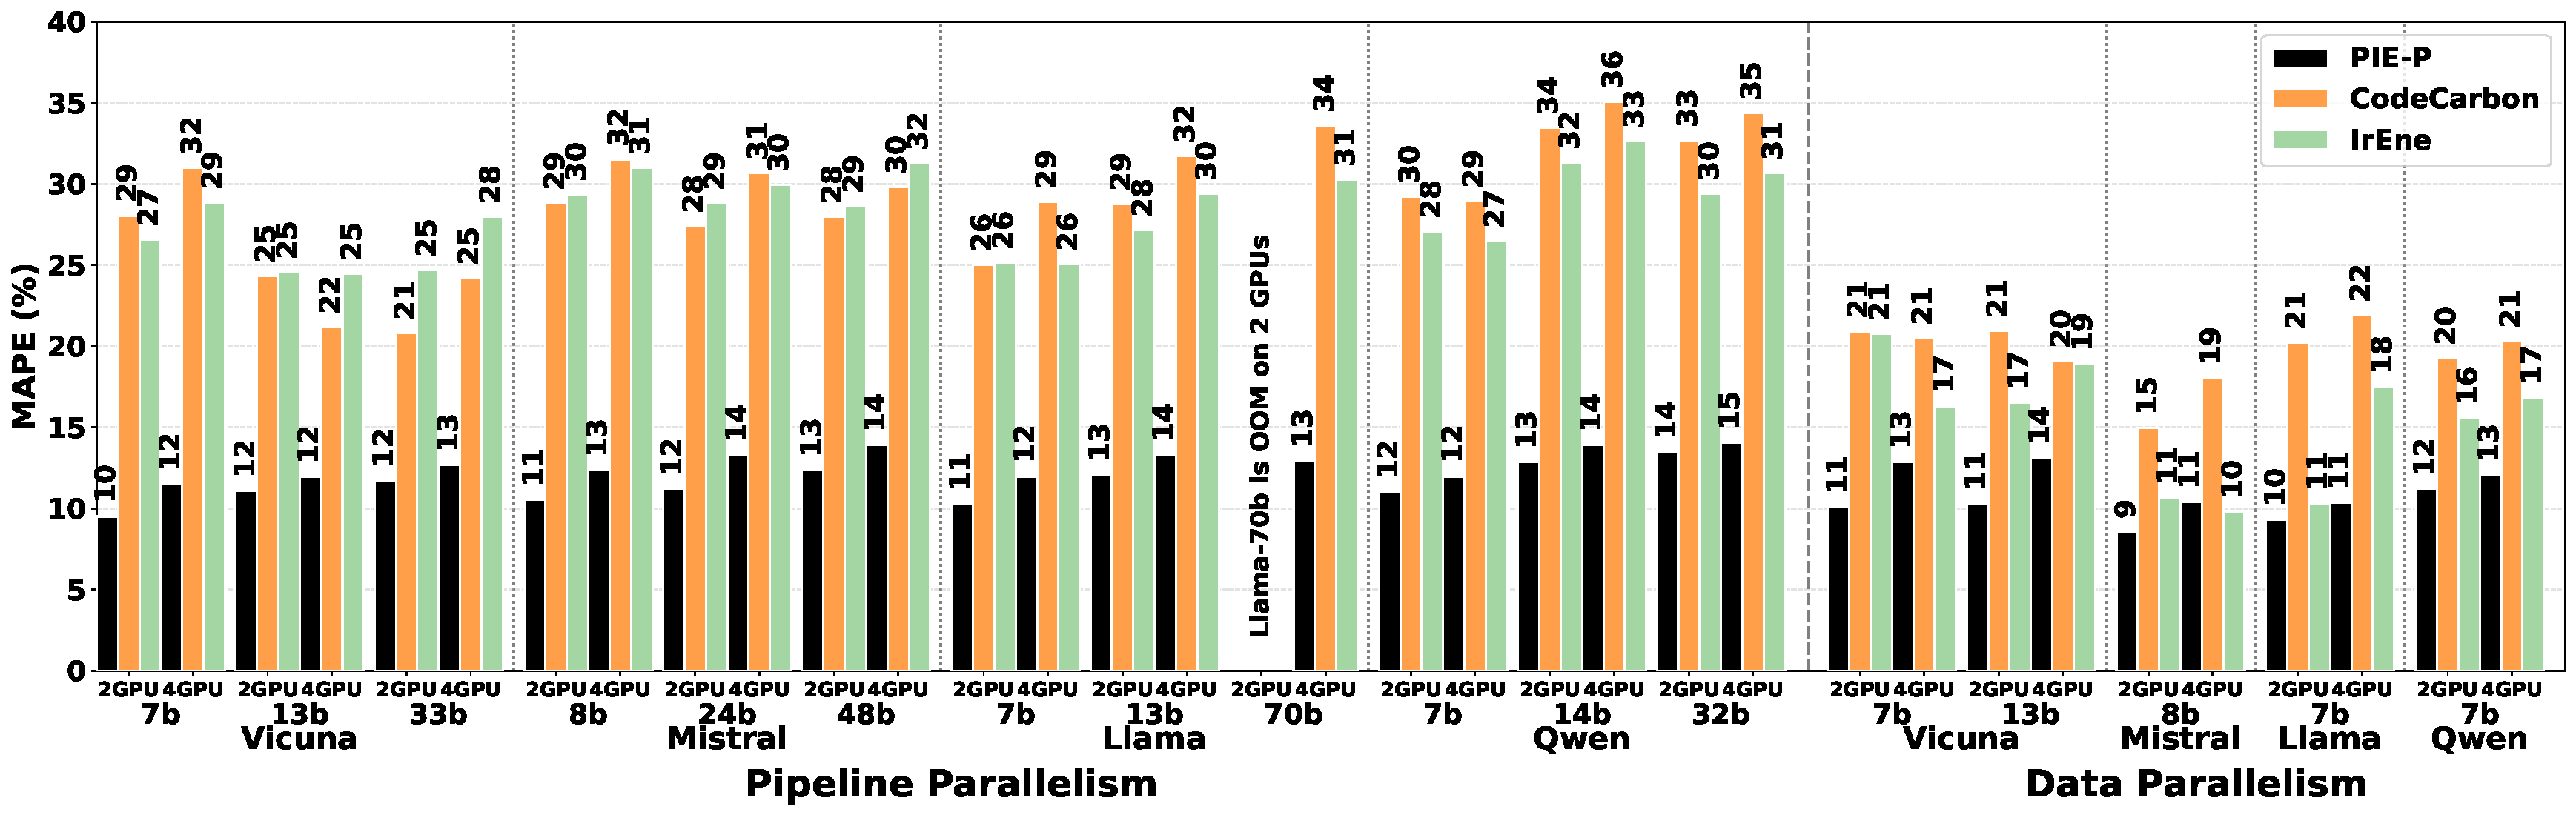
\includegraphics[height=0.22\textwidth,width=0.9\textwidth]{figures/pp_dp_comparison.pdf}
    \vspace{-10pt}
    \caption{MAPE results for all 4 model families under pipeline and data parallelism. Models with the largest parameter sizes in all 4 model families could not be compared for DP as they did not fit in GPU memory.}
    \label{fig:mape_comparison_other}
    \vspace{-18pt}
\end{figure*}

Figure~\ref{fig:mape_comparison_other} compares \sys{} against CodeCarbon and IrEne across all four model families and both 2-GPU and 4-GPU deployments under pipeline and data parallelism. We omit the Wilkins et al.\ baseline as it is consistently inferior to the other baselines (see Figure~\ref{fig:mape_comparison}). We also exclude configurations that do not fit in GPU memory (e.g., Llama-70B on 2 GPUs under pipeline parallelism, and several larger models under data parallelism).

Across all evaluated configurations, \be{\sys{} achieves the lowest prediction error for both parallelism strategies}.
Averaged over all points in Figure~\ref{fig:mape_comparison_other}, \sys{} attains MAPE of 12.2\% under pipeline parallelism and 10.8\% under data parallelism.
The baselines incur higher error: CodeCarbon and IrEne achieve 29.0\% and 28.3\% MAPE under pipeline parallelism, respectively, and 19.6\% and 15.3\% under data parallelism.



Pipeline parallel inference incurs recurring inter-GPU data transfers at every stage boundary.
As the number of GPUs increases (hence more stages), the \emph{frequency} of communication events also increases, making pipeline inference particularly sensitive to unmodeled communication effects.
As a result CodeCarbon and IrEne exhibit large errors, especially under 4-GPU.
Data parallel inference, on the other hand, incurs less frequent and more structured communication.
Thus, the penalty for omitting communication, as in CodeCarbon and IrEne, is smaller than in pipeline parallelism, though still higher than \sys{}.

\review{We use tensor parallelism for the full suite of module-level, leave-one-out, hardware, and ablation experiments because it is the most communication-intensive prediction setting: individual operators are sharded across GPUs and collective communication appears repeatedly inside Transformer blocks. Pipeline parallelism instead communicates activations at stage boundaries, while our data-parallel inference setup has less frequent and more structured output communication. The pipeline- and data-parallel experiments therefore test whether the same \sys{} formulation extends to these different communication structures, while the deeper generalization analysis is concentrated on the more challenging tensor-parallel setting.}

\subsection{Ablation Study: Communication Model}
\label{sec:ablation_comm_modeling}
The \textsc{AvgComm} comparison described in \S\ref{ss:esetup} retains \sys{}'s model-tree decomposition and compute-module predictors while replacing the explicit communication model with an average-power estimate.

\begin{figure*}[t]
    \centering
    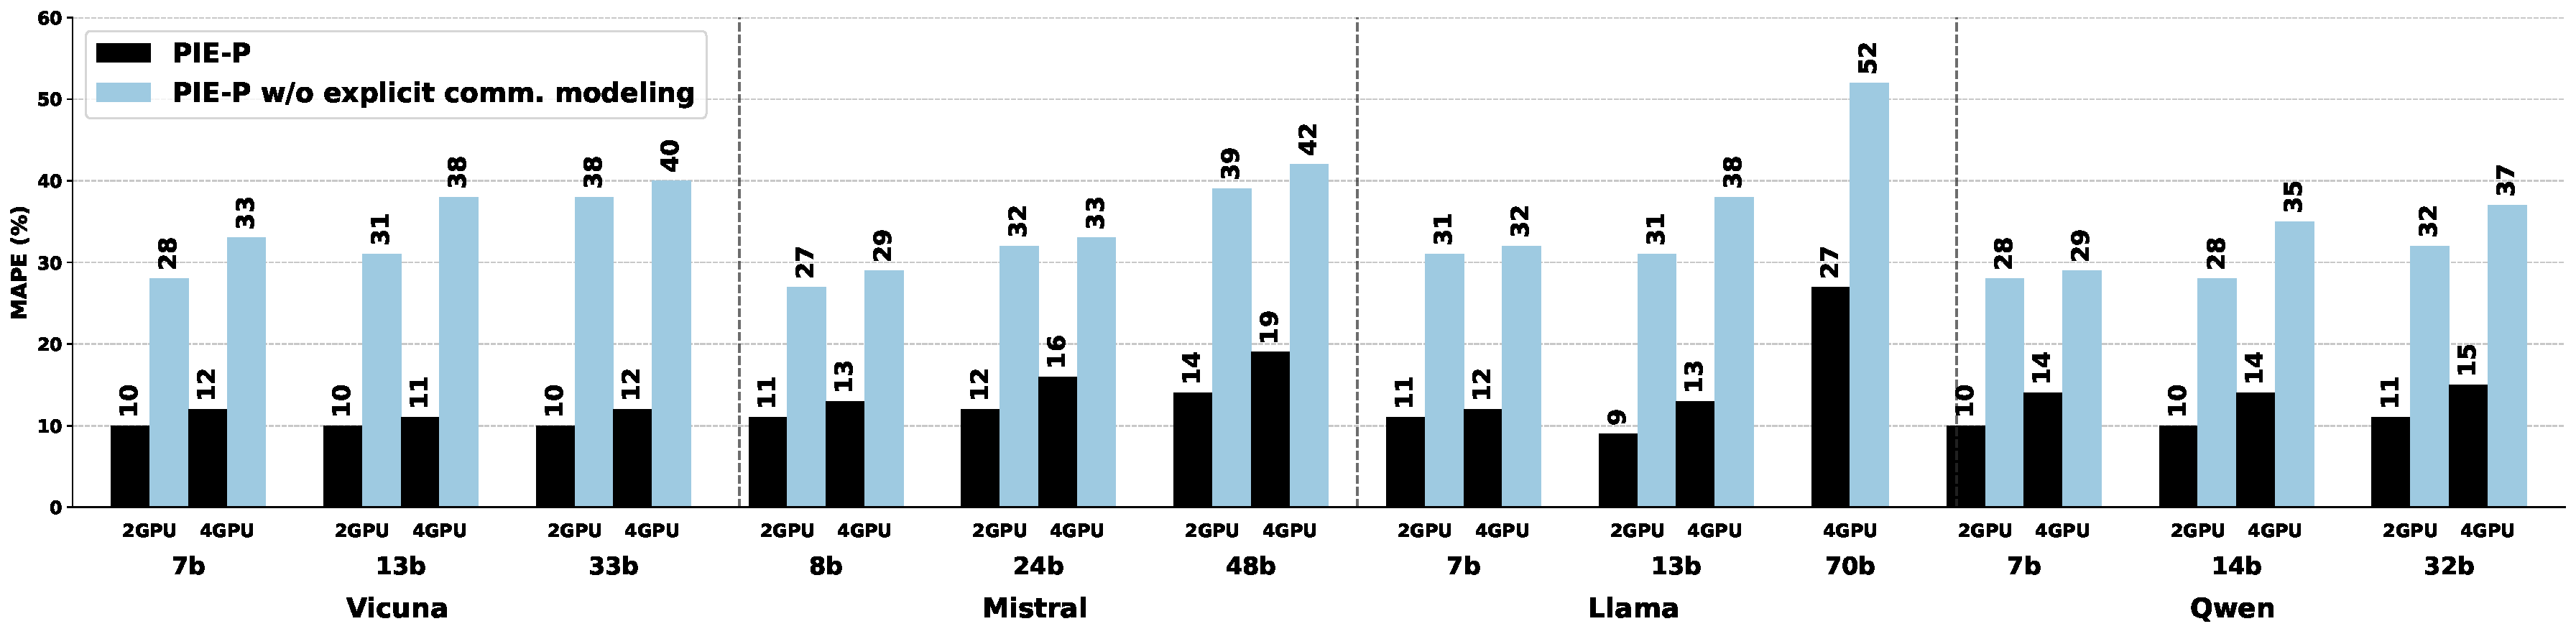
\includegraphics[width=\textwidth]{figures/mape_all_model_families_no_comm_modeling.pdf}
    \vspace{-24pt}
    \caption{Ablation of explicit communication modeling. The ablated variant replaces \sys{}'s communication model with an average communication-power estimate for AllReduce events.}
    \label{fig:ablation_comm_modeling}
    \vspace{-15pt}
\end{figure*}

Figure~\ref{fig:ablation_comm_modeling} shows that \textsc{AvgComm} incurs substantially higher prediction error of 34.0\% compared to \sys{}'s 12.9\%.
The error increase is especially noticeable for larger models and 4-GPU settings, where AllReduce contributes a larger fraction of total energy.
The key distinction is that \sys{} models communication as a first-class module whose features reflect the actual communication.
The \textsc{AvgComm} ablation collapses these differences into a single average value, losing the structure needed to predict communication energy accurately.

\subsection{Ablation Study: Model Tree methodology}
\label{sec:ablation}
We next evaluate the model-level regression comparison described in \S\ref{ss:esetup}, which removes module-level decomposition.

We find that directly predicting total model energy leads to substantially higher errors: the MAPE increases to 61.2\% for Vicuna, 84.3\% for Mistral, 115.1\% for Llama, and 60.8\% for Qwen.
This shows that energy prediction for parallel inference is not simply a model-level regression problem. Runtime features vary significantly across compute-heavy modules (e.g., Attention, MLP) and communication-heavy modules (e.g., AllReduce). Collapsing these effects into a single aggregate feature loses this structure and causes the predictor to mix heterogeneous sources of energy variation.

\anurag{Appendix - K Additional Results: Feature correlation analysis}
\review{\smallskip\noindent\textbf{Feature-correlation analysis.} To assess whether the feature set contributes information beyond one GPU-energy signal, we compute Spearman rank correlations between the candidate features and total measured energy across Vicuna configurations. NVML GPU energy is strongly correlated with total energy ($\rho=0.633$--$0.762$), as expected because GPU computation is a major contributor. However, several non-NVML features are similarly informative: batch size has $\rho=0.735$--$0.737$, execution time has $\rho=0.658$--$0.664$, and memory usage has $\rho=0.656$--$0.663$. Thus, workload size, execution duration, memory activity, and GPU energy all contribute signal; in multi-GPU execution, communication volume and synchronization further perturb these relationships. This supports the multi-feature design rather than a single utilization or telemetry scalar.}

\anurag{Appendix - L Additional Results: Using Latency Prediction Approaches to Predict Energy}
\review{\smallskip\noindent\textbf{Can a latency predictor be retargeted to energy?} Using the NeuSight-style energy predictor described with the baselines above, Table~\ref{tab:neusight_energy_target} shows an average MAPE of 87.3\%, roughly 3--5$\times$ worse than \sys{}. Latency-oriented features describe how long kernels execute but do not explicitly capture power dynamics, system-level energy, inter-GPU communication, or synchronization/waiting effects.}

\begin{table}[t]
\centering
\small
\setlength{\tabcolsep}{6pt}
\renewcommand{\arraystretch}{1.05}
\begin{tabular}{lc}
\toprule
\textbf{Model} & \textbf{MAPE} \\
\midrule
\rowcolor{rowblue} Vicuna 7B  & 79.19\% \\
Vicuna 13B                    & 93.24\% \\
\rowcolor{rowblue} Vicuna 33B & 89.38\% \\
\bottomrule
\end{tabular}
\caption{MAPE for a NeuSight-style latency prediction framework when energy is used as the prediction target.}
\label{tab:neusight_energy_target}
\end{table}

\begin{figure}[t]
    \centering
    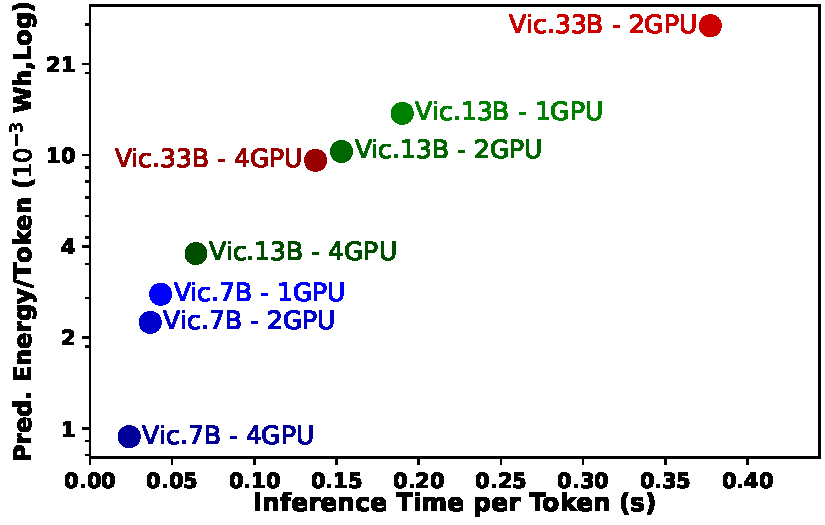
\includegraphics[width=0.40\textwidth]{figures/pareto_plot.pdf}
    \vspace{-9pt}
    \caption{Predicted trade-off between inference time per token and energy per token (log scale) for Vicuna under tensor parallelism.}
    \label{fig:pareto_plot}
    \vspace{-18pt}
\end{figure}
\subsection{Use case: Inference time vs.\ energy for different levels of tensor parallelization}
\label{sec:usecase}

We now present a use case to highlight the applicability of \sys{} in practice.
Consider a setting where an LLM user needs to choose a model and the number of GPUs across which to deploy.
A developer may want to both maximize throughput (i.e., have less time spent on inference per token) and reduce energy consumption.
We show how the user can employ \sys{} to make the right decision.
Figure~\ref{fig:pareto_plot}
illustrates the trade-off between (predicted) energy as a function of inference time for Vicuna models of sizes 7B, 13B, and 33B, across different tensor parallelism configurations (1, 2, and 4 GPUs). We use the highest batch size achievable for each model size. Results are normalized per token and presented on log scale. When compared to ground truth, our prediction errors are around 15\%.

Both per-token energy and inference time increase with model size (7B to 33B), but decrease as the degree of parallelization increases across all three model sizes.
For smaller models such as Vicuna-7B, increasing GPU count from 2 to 4 reduced energy consumption by 43\%, but improved inference time by only 20\%, highlighting diminishing returns. In contrast, larger models like Vicuna-33B benefited more significantly, with a 33\% reduction in energy and a 50\% improvement in speed.
We also extended this analysis to the Qwen family of models, where we found a different scaling efficiency: Qwen-32B achieved 40\% energy reduction when scaling from 2 to 4 GPUs, compared to 33\% for Vicuna-33B, while maintaining similar speedups.

In effect, the energy impact of parallelization is not obvious. Without accurate predictions, model developers require numerous trial-and-error experiments to make energy-conscious parallelization decisions. \sys{} mitigates this effort, providing scalable energy predictions to guide decisions.
